% Options for packages loaded elsewhere
\PassOptionsToPackage{unicode}{hyperref}
\PassOptionsToPackage{hyphens}{url}
\PassOptionsToPackage{dvipsnames,svgnames,x11names}{xcolor}
%
\documentclass[
  letterpaper,
  DIV=11,
  numbers=noendperiod]{scrreprt}

\usepackage{amsmath,amssymb}
\usepackage{iftex}
\ifPDFTeX
  \usepackage[T1]{fontenc}
  \usepackage[utf8]{inputenc}
  \usepackage{textcomp} % provide euro and other symbols
\else % if luatex or xetex
  \usepackage{unicode-math}
  \defaultfontfeatures{Scale=MatchLowercase}
  \defaultfontfeatures[\rmfamily]{Ligatures=TeX,Scale=1}
\fi
\usepackage{lmodern}
\ifPDFTeX\else  
    % xetex/luatex font selection
\fi
% Use upquote if available, for straight quotes in verbatim environments
\IfFileExists{upquote.sty}{\usepackage{upquote}}{}
\IfFileExists{microtype.sty}{% use microtype if available
  \usepackage[]{microtype}
  \UseMicrotypeSet[protrusion]{basicmath} % disable protrusion for tt fonts
}{}
\makeatletter
\@ifundefined{KOMAClassName}{% if non-KOMA class
  \IfFileExists{parskip.sty}{%
    \usepackage{parskip}
  }{% else
    \setlength{\parindent}{0pt}
    \setlength{\parskip}{6pt plus 2pt minus 1pt}}
}{% if KOMA class
  \KOMAoptions{parskip=half}}
\makeatother
\usepackage{xcolor}
\setlength{\emergencystretch}{3em} % prevent overfull lines
\setcounter{secnumdepth}{5}
% Make \paragraph and \subparagraph free-standing
\ifx\paragraph\undefined\else
  \let\oldparagraph\paragraph
  \renewcommand{\paragraph}[1]{\oldparagraph{#1}\mbox{}}
\fi
\ifx\subparagraph\undefined\else
  \let\oldsubparagraph\subparagraph
  \renewcommand{\subparagraph}[1]{\oldsubparagraph{#1}\mbox{}}
\fi

\usepackage{color}
\usepackage{fancyvrb}
\newcommand{\VerbBar}{|}
\newcommand{\VERB}{\Verb[commandchars=\\\{\}]}
\DefineVerbatimEnvironment{Highlighting}{Verbatim}{commandchars=\\\{\}}
% Add ',fontsize=\small' for more characters per line
\usepackage{framed}
\definecolor{shadecolor}{RGB}{241,243,245}
\newenvironment{Shaded}{\begin{snugshade}}{\end{snugshade}}
\newcommand{\AlertTok}[1]{\textcolor[rgb]{0.68,0.00,0.00}{#1}}
\newcommand{\AnnotationTok}[1]{\textcolor[rgb]{0.37,0.37,0.37}{#1}}
\newcommand{\AttributeTok}[1]{\textcolor[rgb]{0.40,0.45,0.13}{#1}}
\newcommand{\BaseNTok}[1]{\textcolor[rgb]{0.68,0.00,0.00}{#1}}
\newcommand{\BuiltInTok}[1]{\textcolor[rgb]{0.00,0.23,0.31}{#1}}
\newcommand{\CharTok}[1]{\textcolor[rgb]{0.13,0.47,0.30}{#1}}
\newcommand{\CommentTok}[1]{\textcolor[rgb]{0.37,0.37,0.37}{#1}}
\newcommand{\CommentVarTok}[1]{\textcolor[rgb]{0.37,0.37,0.37}{\textit{#1}}}
\newcommand{\ConstantTok}[1]{\textcolor[rgb]{0.56,0.35,0.01}{#1}}
\newcommand{\ControlFlowTok}[1]{\textcolor[rgb]{0.00,0.23,0.31}{#1}}
\newcommand{\DataTypeTok}[1]{\textcolor[rgb]{0.68,0.00,0.00}{#1}}
\newcommand{\DecValTok}[1]{\textcolor[rgb]{0.68,0.00,0.00}{#1}}
\newcommand{\DocumentationTok}[1]{\textcolor[rgb]{0.37,0.37,0.37}{\textit{#1}}}
\newcommand{\ErrorTok}[1]{\textcolor[rgb]{0.68,0.00,0.00}{#1}}
\newcommand{\ExtensionTok}[1]{\textcolor[rgb]{0.00,0.23,0.31}{#1}}
\newcommand{\FloatTok}[1]{\textcolor[rgb]{0.68,0.00,0.00}{#1}}
\newcommand{\FunctionTok}[1]{\textcolor[rgb]{0.28,0.35,0.67}{#1}}
\newcommand{\ImportTok}[1]{\textcolor[rgb]{0.00,0.46,0.62}{#1}}
\newcommand{\InformationTok}[1]{\textcolor[rgb]{0.37,0.37,0.37}{#1}}
\newcommand{\KeywordTok}[1]{\textcolor[rgb]{0.00,0.23,0.31}{#1}}
\newcommand{\NormalTok}[1]{\textcolor[rgb]{0.00,0.23,0.31}{#1}}
\newcommand{\OperatorTok}[1]{\textcolor[rgb]{0.37,0.37,0.37}{#1}}
\newcommand{\OtherTok}[1]{\textcolor[rgb]{0.00,0.23,0.31}{#1}}
\newcommand{\PreprocessorTok}[1]{\textcolor[rgb]{0.68,0.00,0.00}{#1}}
\newcommand{\RegionMarkerTok}[1]{\textcolor[rgb]{0.00,0.23,0.31}{#1}}
\newcommand{\SpecialCharTok}[1]{\textcolor[rgb]{0.37,0.37,0.37}{#1}}
\newcommand{\SpecialStringTok}[1]{\textcolor[rgb]{0.13,0.47,0.30}{#1}}
\newcommand{\StringTok}[1]{\textcolor[rgb]{0.13,0.47,0.30}{#1}}
\newcommand{\VariableTok}[1]{\textcolor[rgb]{0.07,0.07,0.07}{#1}}
\newcommand{\VerbatimStringTok}[1]{\textcolor[rgb]{0.13,0.47,0.30}{#1}}
\newcommand{\WarningTok}[1]{\textcolor[rgb]{0.37,0.37,0.37}{\textit{#1}}}

\providecommand{\tightlist}{%
  \setlength{\itemsep}{0pt}\setlength{\parskip}{0pt}}\usepackage{longtable,booktabs,array}
\usepackage{calc} % for calculating minipage widths
% Correct order of tables after \paragraph or \subparagraph
\usepackage{etoolbox}
\makeatletter
\patchcmd\longtable{\par}{\if@noskipsec\mbox{}\fi\par}{}{}
\makeatother
% Allow footnotes in longtable head/foot
\IfFileExists{footnotehyper.sty}{\usepackage{footnotehyper}}{\usepackage{footnote}}
\makesavenoteenv{longtable}
\usepackage{graphicx}
\makeatletter
\def\maxwidth{\ifdim\Gin@nat@width>\linewidth\linewidth\else\Gin@nat@width\fi}
\def\maxheight{\ifdim\Gin@nat@height>\textheight\textheight\else\Gin@nat@height\fi}
\makeatother
% Scale images if necessary, so that they will not overflow the page
% margins by default, and it is still possible to overwrite the defaults
% using explicit options in \includegraphics[width, height, ...]{}
\setkeys{Gin}{width=\maxwidth,height=\maxheight,keepaspectratio}
% Set default figure placement to htbp
\makeatletter
\def\fps@figure{htbp}
\makeatother

\KOMAoption{captions}{tableheading}
\makeatletter
\makeatother
\makeatletter
\@ifpackageloaded{bookmark}{}{\usepackage{bookmark}}
\makeatother
\makeatletter
\@ifpackageloaded{caption}{}{\usepackage{caption}}
\AtBeginDocument{%
\ifdefined\contentsname
  \renewcommand*\contentsname{Table of contents}
\else
  \newcommand\contentsname{Table of contents}
\fi
\ifdefined\listfigurename
  \renewcommand*\listfigurename{List of Figures}
\else
  \newcommand\listfigurename{List of Figures}
\fi
\ifdefined\listtablename
  \renewcommand*\listtablename{List of Tables}
\else
  \newcommand\listtablename{List of Tables}
\fi
\ifdefined\figurename
  \renewcommand*\figurename{Figure}
\else
  \newcommand\figurename{Figure}
\fi
\ifdefined\tablename
  \renewcommand*\tablename{Table}
\else
  \newcommand\tablename{Table}
\fi
}
\@ifpackageloaded{float}{}{\usepackage{float}}
\floatstyle{ruled}
\@ifundefined{c@chapter}{\newfloat{codelisting}{h}{lop}}{\newfloat{codelisting}{h}{lop}[chapter]}
\floatname{codelisting}{Listing}
\newcommand*\listoflistings{\listof{codelisting}{List of Listings}}
\makeatother
\makeatletter
\@ifpackageloaded{caption}{}{\usepackage{caption}}
\@ifpackageloaded{subcaption}{}{\usepackage{subcaption}}
\makeatother
\makeatletter
\@ifpackageloaded{tcolorbox}{}{\usepackage[skins,breakable]{tcolorbox}}
\makeatother
\makeatletter
\@ifundefined{shadecolor}{\definecolor{shadecolor}{rgb}{.97, .97, .97}}
\makeatother
\makeatletter
\makeatother
\makeatletter
\makeatother
\ifLuaTeX
  \usepackage{selnolig}  % disable illegal ligatures
\fi
\IfFileExists{bookmark.sty}{\usepackage{bookmark}}{\usepackage{hyperref}}
\IfFileExists{xurl.sty}{\usepackage{xurl}}{} % add URL line breaks if available
\urlstyle{same} % disable monospaced font for URLs
\hypersetup{
  pdftitle={Intro to Linux},
  pdfauthor={Matthew R. Gemmell},
  colorlinks=true,
  linkcolor={blue},
  filecolor={Maroon},
  citecolor={Blue},
  urlcolor={Blue},
  pdfcreator={LaTeX via pandoc}}

\title{Intro to Linux}
\author{Matthew R. Gemmell}
\date{2023-11-01}

\begin{document}
\maketitle
\ifdefined\Shaded\renewenvironment{Shaded}{\begin{tcolorbox}[sharp corners, boxrule=0pt, borderline west={3pt}{0pt}{shadecolor}, interior hidden, enhanced, frame hidden, breakable]}{\end{tcolorbox}}\fi

\renewcommand*\contentsname{Table of contents}
{
\hypersetup{linkcolor=}
\setcounter{tocdepth}{2}
\tableofcontents
}
\bookmarksetup{startatroot}

\hypertarget{intro}{%
\chapter{Introduction}\label{intro}}

\begin{figure}

{\centering 
\includegraphics[width=0.3\textwidth,height=\textheight]{figures/NEOF.png}

}

\end{figure}

\begin{figure}

{\centering 
\includegraphics[width=0.2\textwidth,height=\textheight]{figures/linux_beginner.png}

}

\end{figure}

Bioinformatics is an increasingly important skill for biological
scientists. Many bioinformatic tools can only be run on Linux based
operating systems. This course aims to introduce you to Linux and is
aimed at beginners and novices to the command line.

Sessions will start with a brief presentation followed by self-paced
computer practicals guided by an online interactive book. The book will
contain theory, practice code, and exercises. Multiple choice questions
will help reinforce what you have learnt throughout the book.

At the end of the course learners will be able to:

\begin{itemize}
\tightlist
\item
  Explain how the user, shell, and kernel interact with each other in
  the Linux OS.
\item
  Navigate \& manipulate directories in the Linux environment.
\item
  List and view the contents of directories.
\item
  Carry out a variety of commands with files including printing them to
  terminal.
\item
  Utilise the text editor nano to create, edit, and save files.
\item
  Understand the structure of fastq files.
\end{itemize}

There are additional materials in chapters 12-14 which include some
advanced Linux commands and introductions to other programming languages
used by bioinformaticians.

Commands are in the following font, colour, and box. They should be run
in the command line.

\begin{Shaded}
\begin{Highlighting}[]
\BuiltInTok{echo} \StringTok{"This is a command example"} 
\end{Highlighting}
\end{Shaded}

In some chapters there are video walk-throughs. These are optional and
give you a guided visual walk-through of running the practice code in
the chapter. These are found in an expandable box at the start of the
chapters 4,5,6, and 8.

Additionally, please use the \protect\hyperlink{cheatsheet}{cheatsheet}
as a reminder of all the commands you will be learning.

\hypertarget{table-of-contents}{%
\section*{Table of contents}\label{table-of-contents}}
\addcontentsline{toc}{section}{Table of contents}

\markright{Table of contents}

\begin{longtable}[]{@{}
  >{\centering\arraybackslash}p{(\columnwidth - 2\tabcolsep) * \real{0.5109}}
  >{\centering\arraybackslash}p{(\columnwidth - 2\tabcolsep) * \real{0.4891}}@{}}
\toprule\noalign{}
\endhead
\bottomrule\noalign{}
\endlastfoot
\begin{minipage}[t]{\linewidth}\centering
\protect\hyperlink{linuxintro}{\textbf{What is Linux?}}

\begin{figure}

{\centering 

\protect\hyperlink{linuxintro}{
\includegraphics[width=1.47917in,height=\textheight]{figures/linux_beginner.png}}

}

\end{figure}
\end{minipage} & \begin{minipage}[t]{\linewidth}\centering
\protect\hyperlink{cluster}{\textbf{Logging in to our teaching VNC}}

\begin{figure}

{\centering 

\protect\hyperlink{cluster}{
\includegraphics[width=1.96875in,height=\textheight]{figures/start.png}}

}

\end{figure}
\end{minipage} \\
\begin{minipage}[t]{\linewidth}\centering
\protect\hyperlink{dirsandfiles}{\textbf{Directories and files}}

\begin{figure}

{\centering 

\protect\hyperlink{dirsandfiles}{
\includegraphics[width=1.30208in,height=\textheight]{figures/directory.png}}

}

\end{figure}
\end{minipage} & \begin{minipage}[t]{\linewidth}\centering
\protect\hyperlink{tipsandtricks}{\textbf{Tips and tricks}}

\begin{figure}

{\centering 

\protect\hyperlink{tipsandtricks}{
\includegraphics[width=3.14583in,height=\textheight]{figures/skateboard_trick.png}}

}

\end{figure}
\end{minipage} \\
\begin{minipage}[t]{\linewidth}\centering
\protect\hyperlink{manipulatingdirectories}{\textbf{Manipulating
Directories}}

\begin{figure}

{\centering 

\protect\hyperlink{manipulatingdirectories}{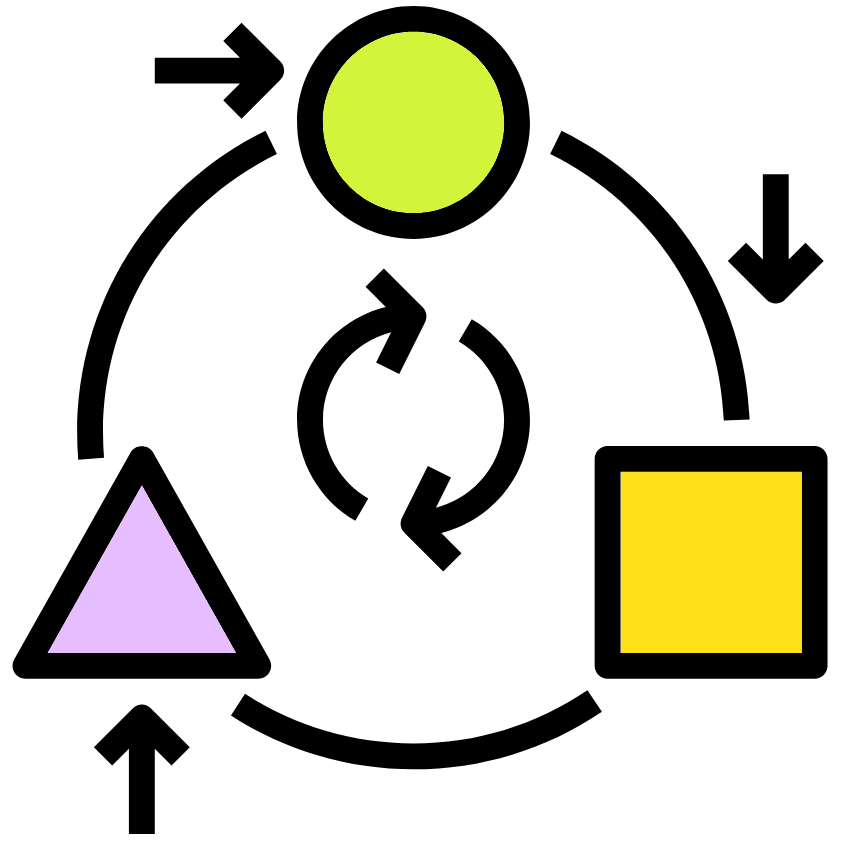
\includegraphics[width=1.5625in,height=\textheight]{figures/transform.png}}

}

\end{figure}
\end{minipage} & \begin{minipage}[t]{\linewidth}\centering
\protect\hyperlink{filereadingandprocessing}{\textbf{File reading and
processing}}

\begin{figure}

{\centering 

\protect\hyperlink{filereadingandprocessing}{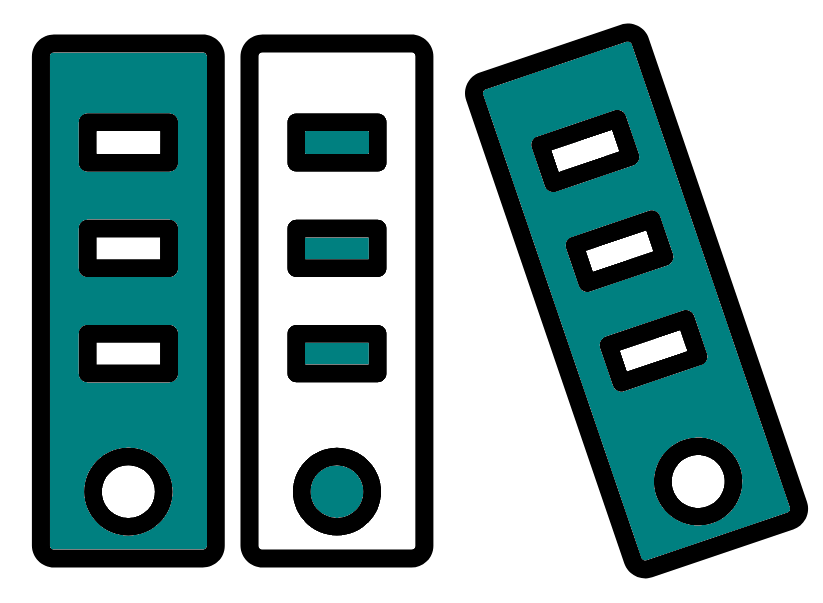
\includegraphics[width=2.13542in,height=\textheight]{figures/files.png}}

}

\end{figure}
\end{minipage} \\
\begin{minipage}[t]{\linewidth}\centering
\protect\hyperlink{advancedlinux}{\textbf{Advanced Linux}}

\begin{figure}

{\centering 

\protect\hyperlink{advancedlinux}{
\includegraphics[width=1.47917in,height=\textheight]{figures/linux_intermdiary.png}}

}

\end{figure}
\end{minipage} & \begin{minipage}[t]{\linewidth}\centering
\protect\hyperlink{bfxlanguages}{\textbf{Other Bioinformatics
programming languages}}

\begin{figure}

{\centering 

\protect\hyperlink{bfxlanguages}{
\includegraphics[width=1.65625in,height=\textheight]{figures/languages.png}}

}

\end{figure}
\end{minipage} \\
\begin{minipage}[t]{\linewidth}\centering
\protect\hyperlink{cheatsheet}{\textbf{Appendix}}

\begin{figure}

{\centering 

\protect\hyperlink{cheatsheet}{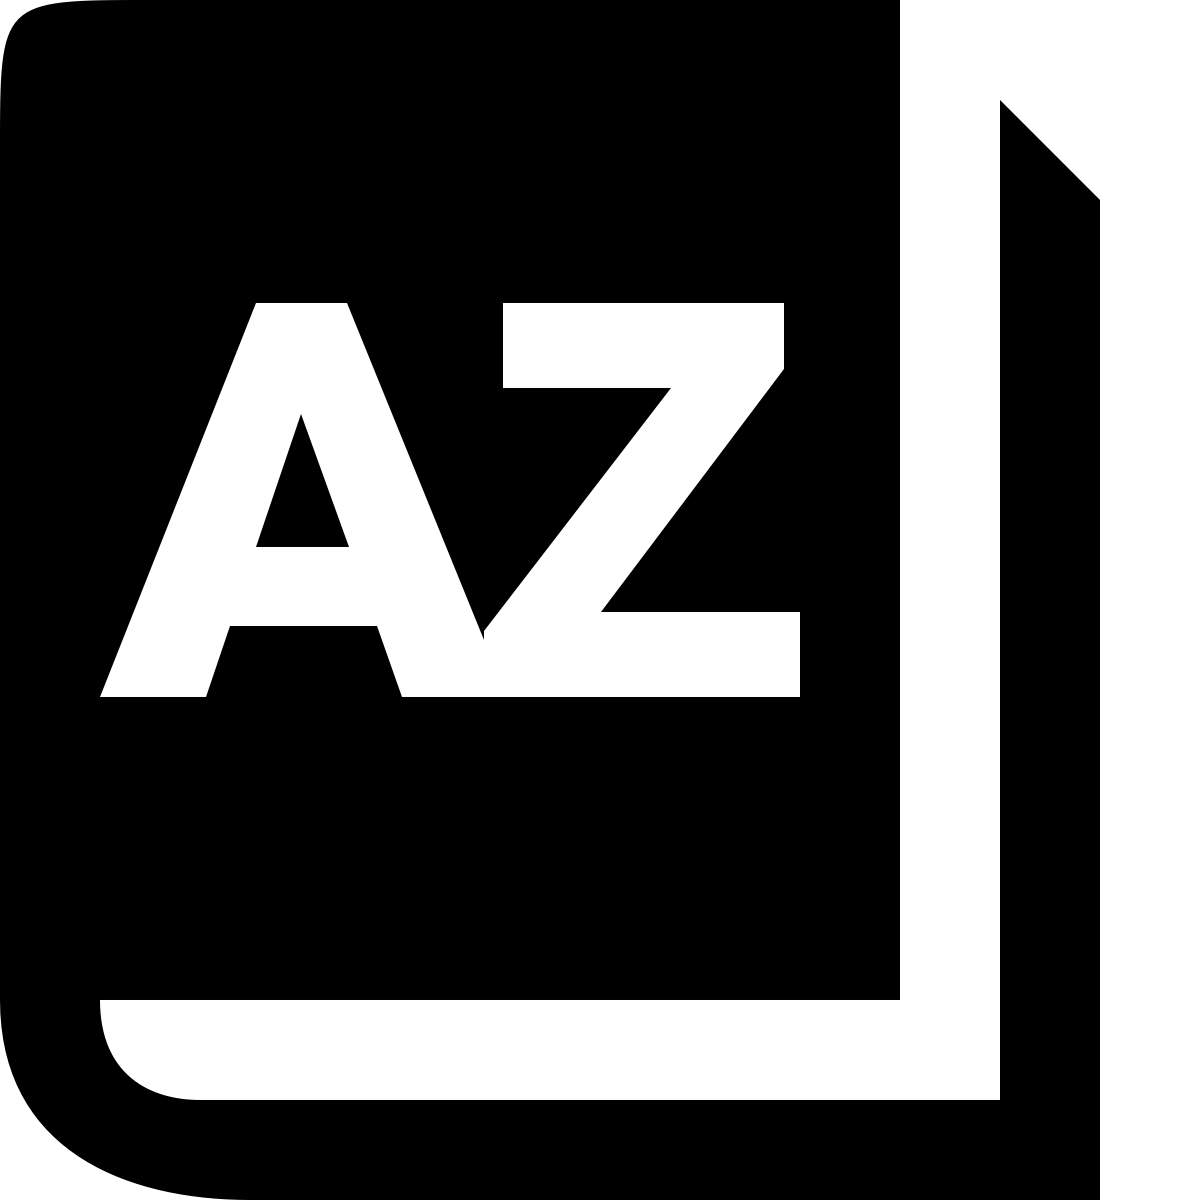
\includegraphics[width=1.5625in,height=\textheight]{figures/cheatsheet.png}}

}

\end{figure}
\end{minipage} & \\
\end{longtable}

This work is licensed under a Creative Commons
Attribution-NonCommercial-ShareAlike 4.0 International License.

\bookmarksetup{startatroot}

\hypertarget{part-part-1}{%
\chapter*{(PART*) Part 1}\label{part-part-1}}
\addcontentsline{toc}{chapter}{(PART*) Part 1}

\markboth{(PART*) Part 1}{(PART*) Part 1}

\bookmarksetup{startatroot}

\hypertarget{linuxintro}{%
\chapter*{Linux}\label{linuxintro}}
\addcontentsline{toc}{chapter}{Linux}

\markboth{Linux}{Linux}

\begin{figure}

{\centering 
\includegraphics[width=0.2\textwidth,height=\textheight]{figures/linux_beginner.png}

}

\end{figure}

Linux is a multitasking, multiuser Unix-like computer operating system
(OS). Linux can run many different applications (multitasking) and it
can be used by many different people (multiuser) on the same computer at
the same time.

It is utilised by many programmers, including Bioinformaticians. It is a
relatively easy OS to run commands and develop software for. The vast
majority of programs and tools for computational analysis of biological
data will work in Linux.

There are three parts of the Linux OS:

\begin{itemize}
\tightlist
\item
  \textbf{The kernel}: This is the hub of the operating systems. This is
  the ``behind the scenes'' part of the OS which allocates time and
  memory to programs. This controls the hardware.
\item
  \textbf{The shell}: This acts as the interface between the user and
  the kernel. When a user runs commands, the shell will interpret these
  commands for the kernel. The shell can be any program that constitutes
  the user interface e.g.~command line, internet browser, start menu
  etc.
\item
  \textbf{Programs}: Programs allow the OS to perform specific tasks.
  Examples of programs include Internet browsers, genome assembly tools,
  text editors etc.
\end{itemize}

\begin{figure}

{\centering 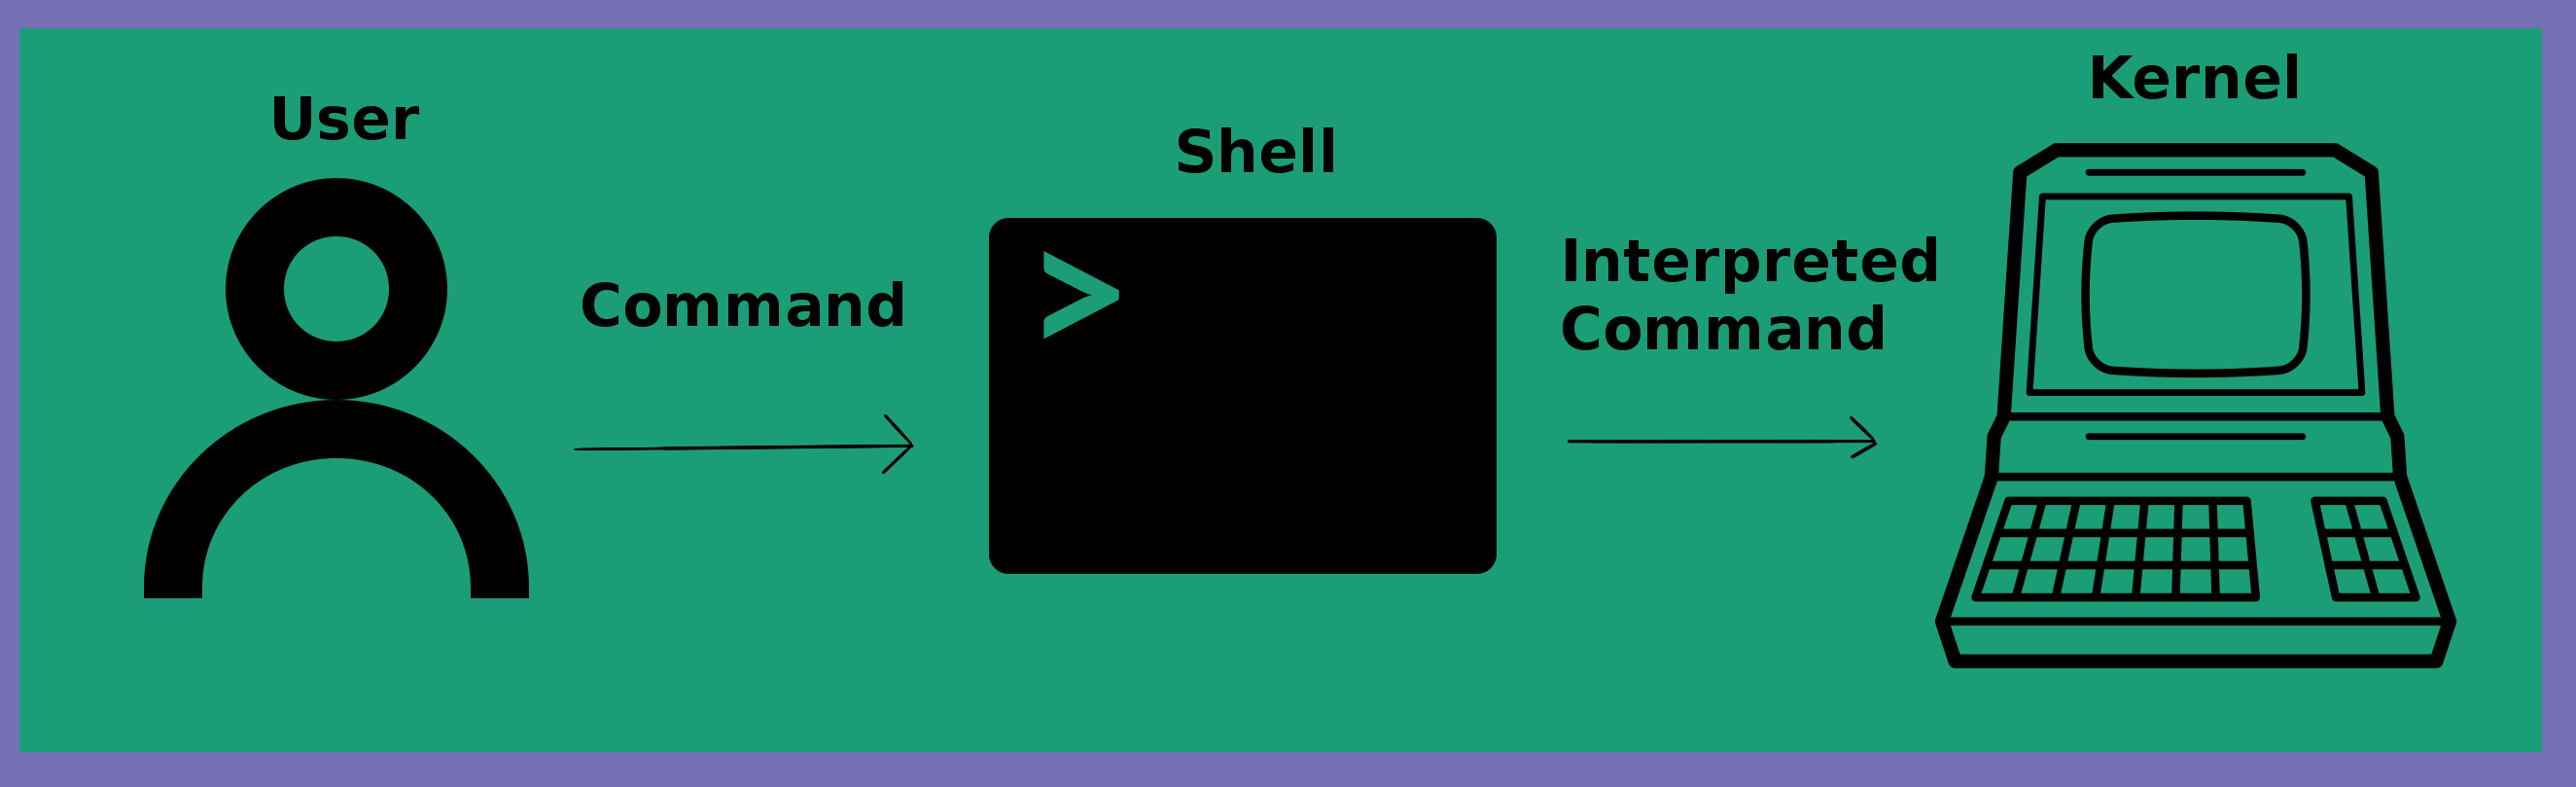
\includegraphics[width=0.8\textwidth,height=\textheight]{figures/linux_user_to_kernel.png}

}

\end{figure}

It is important to learn the Linux language so you can run commands on
the command line. This is because:

\begin{itemize}
\tightlist
\item
  Many bioinformatic tools do not have a graphical user interface (gui)
  and so must be run on the command line.
\item
  There are many powerful commands that can be run on the Linux command
  line.
\item
  It is quicker and more reproducible to run commands through a shell
  than through a gui.
\end{itemize}



\end{document}
